% arara: xelatex: { synctex: true, shell: yes, action: nonstopmode, options: "-halt-on-error" }
% arara: clean: { files: [ report.aux, report.bbl, report.bcf, report.blg, report.log, report.out, report.run.xml ]}
\documentclass{article}
\usepackage[a4paper, margin=1in]{geometry}
\usepackage[utf8]{inputenc}

\usepackage{hyperref}
\usepackage{fontspec}
\setmainfont{Merriweather}
\setmonofont{SpaceMono Nerd Font}

\usepackage{graphicx}
\graphicspath{{img/}}

\usepackage{xcolor}
\definecolor{codebg}{HTML}{222222}

\usepackage{minted}
\usemintedstyle{monokai}

\title{Web Scraping}
\author{Matt Bell}

\begin{document}
\maketitle

\section*{Crowdcube}
The Crowdcube investments page (\url{https://www.crowdcube.com/investments})
contains a list of all deals on the website at any given time. However, it uses
infinite scrolling, so the only way to all of the deals on the page is to keep
scrolling down the page. So one way of solving this would be to use Cheerio
along with something like Phantom.JS to load the page headlessly and to scroll
down the page when all the items are found. Luckily for us, all the data is
stored inside the section tags, almost like they \textit{want} the site to be
scraped. The first inner child is an anchor tag that points to the opportunity
page for more information.

\begin{minted}[breaklines,bgcolor=codebg]{html}
<section class="cc-card" data-="" data-opportunity-id="21421" data-opportunity-name="Redchurch Brewery" data-opportunity-raised="148660" data-opportunity-progress="37" data-opportunity-investors="353" data-opportunity-equity="7.41">
        <!-- some HTML -->
    </section>
\end{minted}

However, I found an interesting API call being made in the network panel as I
was scrolling down.

\begin{figure}[h]
    \centering
    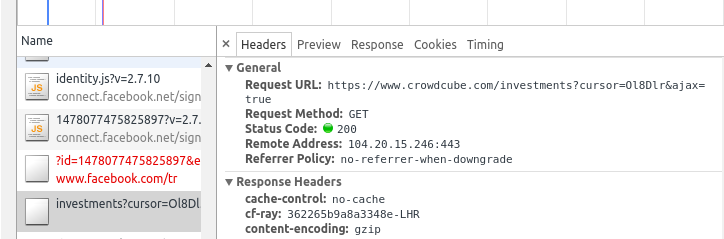
\includegraphics[scale=0.5]{cc_json}
\end{figure}

Making this request with cURL gave me the investments page again, so clearly
there were some methods implemented to prevent scrapers. Looking at the request
made in Chrome, there's a \texttt{x-requested-with} header, set to
\texttt{XMLHTTPRequest}. This value refers to the Javascript browser command
that's used for AJAX calls in the browser. I added it to cURL and got a length
JSON file back.

\begin{minted}[breaklines,bgcolor=codebg]{cl}
    curl -XGET -H "x-requested-with:XMLHttpRequest" https://www.crowdcube.com/investments\?
\end{minted}

\begin{minted}[breaklines,bgcolor=codebg]{json}
    {
        "content": "HTML divs representing the 'opportunities'",
        "cursorNext": "abc012"
    }
\end{minted}

This is a super easy way of bypassing the page scrolling completely\ldots the
\texttt{cursorNext} attribute is the id of the next investment opportunity in
the list. So in the next request, you'd add \texttt{cursor=<cursorNext>} to the
URL string.

\subsection*{Images}
Inside each investment ``card'', there are a few image tags which can be easily
found using CSS selectors.

The logo is using the class \texttt{cc-card\_\_emblemImage}, while the cover
image is shown as the background image of the ``cover'' of the
card\textemdash~which is given the class \texttt{cc-card\_\_cover}.

\section*{Seedrs}
The invest page (\url{https://www.seedrs.com/invest}) contains a list of all the
current investment opportunities. Unlike Crowdcube, the Seedrs site uses static
pagination. This means that each page is accessed using a URL query parameter,
\texttt{page=<1..n>}. Seedrs doesn't set the HTTP response code correctly, so if
you go beyond the number of pages available you'll still receive a 200 OK
response, so you'd have to check for no matching elements on the page.

We can find the list of opportunities on the page by searching for articles with
the class \texttt{CampaignCard}. Each element looks a bit like this:

\begin{minted}[breaklines,bgcolor=codebg]{html}
    <article class="CampaignCard">
        <a href="/morpher" class="Card-link" data-campaign-id="6328" data-campaign-name="Morpher - Folding Helmet Tech" data-campaign-type="equity" data-campaign-categories="Travel, Leisure &amp; Sport, Non-Digital, Mixed B2B/B2C" data-campaign-state="cooling_off_investment">
            <header>
                <div class="Card-cover">
                    <span>
                        <img data-src="https://some-url-to-an-img.png" />
                    </span>
                </div>
                <div class="CampaignCard-campaignLogo">
                    <span>
                        <img data-src="https://some-url-to-an-img.png" />
                    </span>
                </div>
            </header>
            
            <p class="CampaignCard-campaignSummary">
                "Some description"
            </p>
            <ul class="CampaignCard-stats">
                <!-- stats -->
            </ul>
        </a>
    </article>
\end{minted}

This is a little more difficult to parse because of the irregular class naming
scheme and very unclear syntax. Simple information about the opportunity is
stored inside the anchor tag, such as the permalink, name, and categories. The
cover image and logo can be found by looking at the only img tags inside the
\texttt{Card-cover} and \texttt{CampaignCard-campaignLogo} divs respectively. It
seems like the actual image is loaded in dynamically on page load, so the
scraper will probably have to access the \texttt{data-src} attribute to find the
image.

The content of the \texttt{CampaignCard-campaignSummary} div is the summary of
the investment. The statistics are a lot harder to parse. As long as the
campaign type is ``equity'', there are three different
\texttt{CampaignCard-stats} children elements. The first one is the equity
percentage, the second is the investment goal, and the last one is the number of
investors. These can be accessed using the \texttt{CampaignCard-statValue}
class. Most information on the description page is unfortunately protected
behind a login, so the solution is to sign up for an account for the scraper,
and then to use a headless browser like PhantomJS, CasperJS or Selenium.

\section*{Property Partner}
Each property on the page is a list item (class: \texttt{property}), and all of
the properties are present which makes things very easy in terms of pagination.
Inside that list item is an anchor tag with a link to the property's permalink.
From here, we can easily just use CSS selectors inside the element to find the
information we want:

\begin{minted}[breaklines,bgcolor=codebg]{js}
    $('.address h4'); // the address of the property.
    $('.address-detail'); // further information about the property address.
    $('.building'); // description of the building
    $('.tenure'); // details about the tenure e.g. freehold

    $('.image'); // the style attribute contains link to image url.
    $('.funded'); // text value contains the total funded so far.
    $('.target'); // the funding target.
    $('.investors .value'); // the number of current investors
    
    $('.pct-funded value'); // the percentage funding the property has
    $('.time-left'); // time left, in a fuzzy format (e.g. 1 hour, 1 day)
    $('.yield .value'); // the percentage dividend yield
    $('.hpi .value'); // the HPI (house price increase) of the property
\end{minted}

So compared to the previous two websites, Property Partner is rather trivial to
scrape data from. On top of that, the property page groups each piece of data
with a div containing a \texttt{data-expandable} attribute, e.g.
\texttt{preorderDetail} includes information about a pre-order property.
Unfortunately, it looks like the carousel of images is loaded in dynamically
using a minified AngularJS script, so the easiest way of obtaining those would
be to load the webpage using a headless browser.

\section*{Detection Avoidance}
The easiest way to avoid detection is to set request headers to appear to be a
legitimate web browser rather than a headless web scraper. Such headers would
be:
\begin{itemize}
    \item \texttt{user-agent} - a user-agent header specifies the version and
        type of web browser. This can be spoofed to a real user
        agent\textemdash~for instance \texttt{Mozilla/5.0 (X11; Linux x86\_64)
            AppleWebKit/537.36 (KHTML, like Gecko) Chrome/58.0.3029.110
            Safari/537.36}
    \item \texttt{referer} - the referer header specifies the URL that this
        request was sent from. Setting this to website's url means that it
        will look more like a legitimate request.
\end{itemize}

If you want to get extremely in-depth, you could also use a headless browser
(like Phantom.JS) or cURL (with the \texttt{--cookie-jar} option) to store
various session cookies and send those along with the requests to the page. This
way, it looks even more like a legitimate browser request.

Finally, it may be worth\ldots diversifying\ldots your scraping machines. Making
lots of requests from one machine is going to look very suspicious. Acquiring
virtual private servers in a variety of locations, running the scraper and then
destroying them means that the IP addresses used to access the site will be
varying a lot. You could even switch between various cloud providers so that the
acquired IP addresses belong to different network blocks (cloud providers
normally take out a range of IP addresses which your virtual server's address is pooled
from).
This, however, comes with the risk of sending concurrent requests to a single
website which is a great way of accidentally causing a denial of service. So a
possible solution for this is to set up a controlling server, which sends
commands out to the various scrapers to request certain data from the site. This
means that you can at least have one central server that isn't being destroyed,
and it can also store the information collected in a database.

\section*{Testing}
Clearly it would not be a great idea to keep sending requests to the live server
for data when testing. The best option would be to create local copies of the
web pages, manually reduce the number of properties/investments on the page to a
small number, and then manually parse the data. Web requests to the site would
then be ``mocked'', and the local pages would be returned to the scraper to be
tested. API calls could also be mocked in this way. The generated data would
then be compared with the test values. This could be automated using standard
testing libraries like Chai/Mocha.

\end{document}

% vim:set ft=tex textwidth=80 spell:
